% This must be in the first 5 lines to tell arXiv to use pdfLaTeX, which is strongly recommended.
\pdfoutput=1
% In particular, the hyperref package requires pdfLaTeX in order to break URLs across lines.

\documentclass[11pt]{article}

% Remove the "review" option to generate the final version.
% \usepackage[review]{MAIN}
\usepackage[]{MAIN}

% Standard package includes
\usepackage{times}
\usepackage{latexsym}

% For proper rendering and hyphenation of words containing Latin characters (including in bib files)
\usepackage[T1]{fontenc}
% For Vietnamese characters
% \usepackage[T5]{fontenc}
% See https://www.latex-project.org/help/documentation/encguide.pdf for other character sets

% This assumes your files are encoded as UTF8
\usepackage[utf8]{inputenc}

% This is not strictly necessary, and may be commented out.
% However, it will improve the layout of the manuscript,
% and will typically save some space.
\usepackage{microtype}

% This is also not strictly necessary, and may be commented out.
% However, it will improve the aesthetics of text in
% the typewriter font.
\usepackage{inconsolata}

% Used for including images
\usepackage{graphicx}

% Better visual effect of hyper-links
\usepackage{hyperref}
\usepackage{xcolor}
\usepackage{color}
\hypersetup{
    colorlinks,
    linkcolor={red!50!black},
    citecolor={blue!50!black},
    urlcolor={blue!80!black}
}

\usepackage{fancyhdr}

\pagestyle{fancy}
\fancyhf{} % Clear existing header and footer
\fancyfoot[C]{\thepage} % Place the page number in the center of the footer


% If the title and author information does not fit in the area allocated, uncomment the following
%
%\setlength\titlebox{<dim>}
%
% and set <dim> to something 5cm or larger.

\title{Community Detection and Analysis on DBLP v9 Dataset: Centrality, Network Metrics, and Predictive Modeling}

% Author information can be set in various styles:
% For several authors from the same institution:
% \author{
%   Author 1 \and ... \and Author n \\
%   Address line \\ ... \\ Address line
% }
% if the names do not fit well on one line use
%         Author 1 \\ {\bf Author 2} \\ ... \\ {\bf Author n} \\
% For authors from different institutions:
\author{
  Xiang Zheng \\ 21307110169 \And  
  ... 
  \vspace{0.7cm} \\ % Add some space before the school name
  \hfill School of Data Science, Fudan University \hfill
  \And
  Author n \\ Address line
}

\begin{document}
\maketitle
\begin{abstract}
	abstract
\end{abstract}

\section{Introduction}

Network analysis has become an essential methodology for investigating complex systems across diverse domains. The \href{https://www.aminer.cn/citation}{DBLP dataset}, a comprehensive bibliographic repository of computer science publications, provides a rich foundation for exploring collaboration patterns and scholarly relationships. This project employs advanced graph analysis techniques to uncover the structural and functional properties of the DBLP v9 dataset.

The study is organized into five core components, each addressing a key aspect of network analysis:

\begin{itemize}
	\item \textbf{Preprocessing}: The raw DBLP dataset was transformed into a structured network by performing data cleaning, filtering, and splitting. Key preprocessing steps included handling missing data, defining nodes and edges, and attributing properties to network elements to prepare the dataset for analysis.
	\item \textbf{Community Detection}: Cohesive subgroups within the network were identified using algorithms such as Louvain, Label Propagation, and Multi-level. These communities reveal collaborative dynamics, research specializations, and the structural foundations of scholarly interactions.
	\item \textbf{Centrality Analysis}: Degree centrality and PageRank centrality were employed to identify influential nodes, revealing hubs and authoritative figures within the network. Additional metrics, including community diameters and average citations per author, were analyzed to characterize structural and functional network properties. The degree distribution was assessed to evaluate the network's topology, with visual representations provided in the visualization section.
	\item \textbf{Link Prediction}: The GLACE model was employed on the Cora-ML dataset, a citation network of machine learning research papers, to predict potential future connections between nodes. Structural features such as common neighbors and Jaccard similarity served as input, with the model’s performance assessed using metrics like AUC and AP. This analysis offers insights into evolving citation patterns and the dynamics of scholarly connectivity.
	\item \textbf{Visualization System}: An intuitive visualization system was developed to facilitate the interpretation of results. Built using \textbf{Python} for the core implementation and \textbf{D3.js} for dynamic and interactive visualization, the system presents community structures, central nodes, and network statistics through graphical representations. This approach offers a comprehensive and visually accessible overview of the network's topology and dynamics.
\end{itemize}

By integrating these analytical components, this study aims to elucidate the structural characteristics, key actors, and potential evolution of the DBLP co-authorship and publication network. The methodologies and findings presented contribute to a deeper understanding of scholarly collaboration patterns and academic network dynamics.



\section{Preprocessing}

The preprocessing phase is essential for transforming the raw DBLP V9 dataset into a structured format suitable for in-depth analysis. This stage includes data cleaning, network construction, and feature engineering. The DBLP V9 dataset was selected due to its balanced computational efficiency and the required level of detail to explore academic collaboration dynamics. Furthermore, its extensive coverage of computer science literature ensures the robustness of subsequent analyses.

\subsection{Dataset Selection}

The DBLP-Citation-network V9 dataset was chosen for its optimal balance between data richness and computational feasibility, as outlined in Table \ref{tab:dblp_citation_networks}. While earlier versions of the DBLP dataset offer valuable data, V9 strikes a favorable balance between dataset size and manageability, making it well-suited to the available computational resources.

\begin{table*}[h!]
	\centering
	\begin{tabular}{|c|c|c|c|}
		\hline
		\textbf{Dataset}         & \textbf{\# Papers} & \textbf{\# Citation Relationships} & \textbf{Comment}           \\
		\hline
		Citation-network V1       & 629,814            & >632,752                           &                            \\ \hline
		Citation-network V2       & 1,397,240          & >3,021,489                         &                            \\ \hline
		DBLP-Citation-network V3  & 1,632,442          & >2,327,450                         &                            \\ \hline
		DBLP-Citation-network V4  & 1,511,035          & 2,084,019                          & Arnetminer [2011-01-08]    \\ \hline
		DBLP-Citation-network V5  & 1,572,277          & 2,084,019                          & Arnetminer [2011-02-21]    \\ \hline
		DBLP-Citation-network V6  & 2,084,055          & 2,244,018                          & Arnetminer [2013-09-29]    \\ \hline
		DBLP-Citation-network V7  & 2,244,021          & 4,354,534                          & Arnetminer [2014-05-25]    \\ \hline
		DBLP-Citation-network V8  & 3,272,991          & 8,466,859                          & Arnetminer [2016-07-14]    \\ \hline
		ACM-Citation-network V8   & 2,381,688          & 10,476,564                         & Arnetminer [2016-04-02]    \\ \hline
		ACM-Citation-network V9   & 2,385,022          & 9,671,893                          & Arnetminer [2017-01-20]    \\ \hline
		DBLP-Citation-network V9  & 3,680,007          & 1,876,067                          & Arnetminer [2017-07-03]    \\ \hline
		DBLP-Citation-network V10 & 3,079,007          & 25,166,994                         &                            \\ \hline
		DBLP-Citation-network V11 & 4,107,340          & 36,624,464                         & OAG [2019-05-05]           \\ \hline
		DBLP-Citation-network V12 & 4,894,081          & 45,564,149                         & DBLP+Citation [2020-04-09] \\ \hline
		DBLP-Citation-network V13 & 5,354,309          & 48,227,950                         & DBLP+Citation [2021-05-14] \\ \hline
		DBLP-Citation-network V14 & 5,259,858          & 36,630,661                         & DBLP+Citation [2023-01-31] \\
		\hline
	\end{tabular}
	\caption{Summary of DBLP Citation Network Versions}
	\label{tab:dblp_citation_networks}
\end{table*}

DBLP-Citation-network V9 was selected for the following reasons:

\begin{itemize}
	\item \textbf{Data Completeness:} V9 includes 3,680,007 papers and 1,876,067 citation relationships, providing a comprehensive yet manageable dataset.
	\item \textbf{Timeliness:} Released on July 3, 2017, V9 captures citation trends up to that point.
	\item \textbf{Balanced Size:} Compared to later versions, V9 offers a good compromise between data volume and computational feasibility.
	\item \textbf{Sufficient Coverage:} V9’s size facilitates wide-ranging analysis of academic collaborations and citation patterns.
\end{itemize}

Thus, DBLP-Citation-network V9 was selected for its data richness and computational efficiency, making it an ideal candidate for this study.

\subsection{Data Cleaning and Integration}

The raw dataset contains metadata such as titles, authors, venues, and citations. The data cleaning process involved grouping records by paper, resolving missing or inconsistent data, and addressing redundancies. Missing fields, including titles, authors, and venues, were assigned default values to ensure consistency, preparing the dataset for further analysis.

\subsection{Network Construction}

The dataset was structured as a bipartite graph, where authors are represented as nodes and co-authorships as edges. Attributes such as publication count and co-authorship frequency were assigned to the nodes and edges, respectively. Additionally, citation relationships were extracted to construct a directed citation network. This dual representation of collaboration and citation dynamics enables comprehensive analysis of academic interactions.

\subsection{Feature Engineering}

Several key features were engineered to enhance the dataset's analytical power:

\begin{itemize}
	\item \textbf{Co-authorship Mapping:} Authors were assigned unique identifiers, and co-authorship relationships were mapped, with edge weights representing collaboration frequency.
	\item \textbf{Citation Analysis:} Citation relationships were used to calculate in-degree (citations received) and out-degree (citations made) for each paper, offering insights into academic influence and impact.
	\item \textbf{Venue Indexing:} Publication venues were indexed to ensure uniform representation, enabling venue-specific analyses.
\end{itemize}

\subsection{Dataset Filtering}

To improve computational efficiency, papers with no citations or references were flagged as isolates and excluded from analysis. Additionally, thresholds were applied to prioritize significant relationships, ensuring that only meaningful data were retained for subsequent analysis.

\subsection{Overview of the Dataset}

Following preprocessing, a series of exploratory analyses were conducted using Jupyter Notebooks, pandas, and matplotlib to understand the fundamental characteristics and structure of the dataset. The visualizations presented in Figure \ref{fig:num_authors_per_paper}, \ref{fig:citation_distribution}, \ref{fig:reference_distribution}, and \ref{fig:num_coauthors_per_author} summarize key aspects of academic collaboration and citation dynamics, providing insights into author networks, citation patterns, reference behaviors, and co-authorship structures.

\begin{figure*}[h!]
	\centering
	\begin{minipage}{0.24\textwidth}
		\centering
		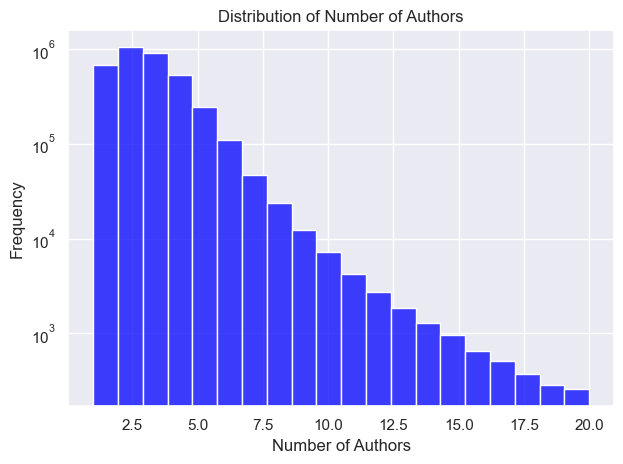
\includegraphics[width=\textwidth]{img/preprocess/num_authors.png}
		\caption{Number of Authors per Paper}
		\label{fig:num_authors_per_paper}
	\end{minipage} \hfill
	\begin{minipage}{0.24\textwidth}
		\centering
		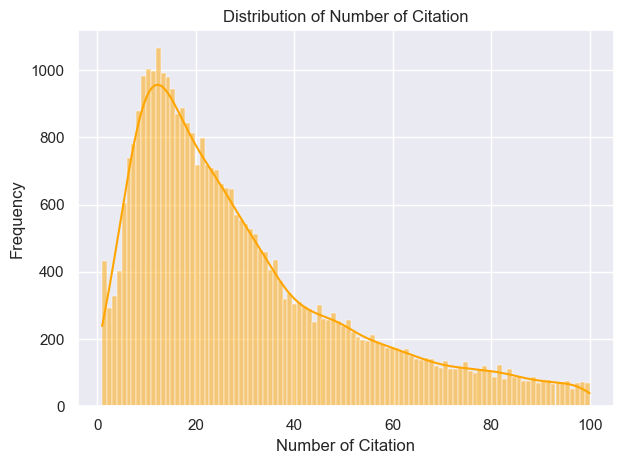
\includegraphics[width=\textwidth]{img/preprocess/num_citations.png}
		\caption{Citation Distribution of Papers}
		\label{fig:citation_distribution}
	\end{minipage} \hfill
	\begin{minipage}{0.24\textwidth}
		\centering
		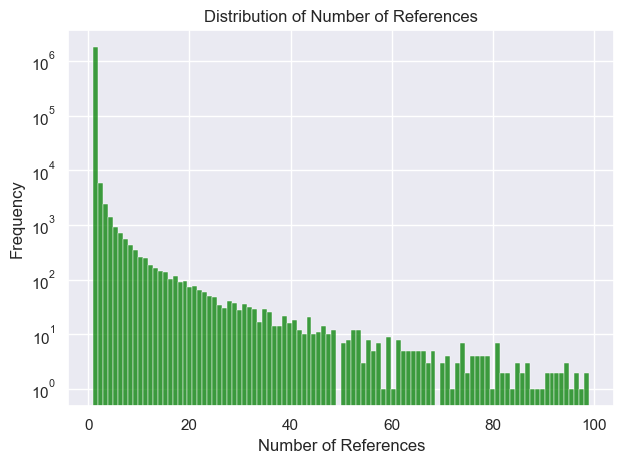
\includegraphics[width=\textwidth]{img/preprocess/num_references.png}
		\caption{Reference Distribution of Papers}
		\label{fig:reference_distribution}
	\end{minipage} \hfill
	\begin{minipage}{0.24\textwidth}
		\centering
		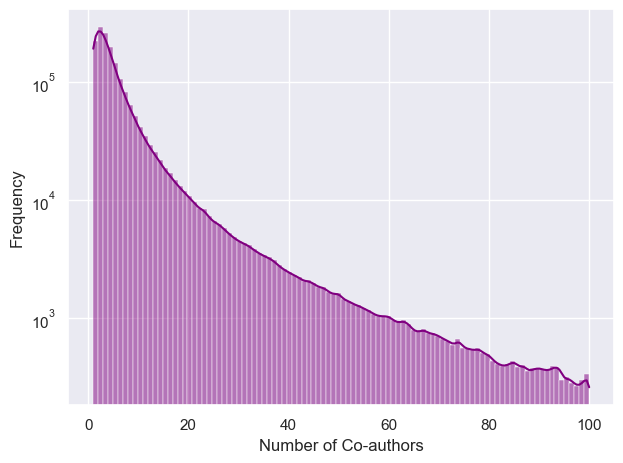
\includegraphics[width=\textwidth]{img/preprocess/num_coauthors.png}
		\caption{Number of Co-authors per Author}
		\label{fig:num_coauthors_per_author}
	\end{minipage} 
\end{figure*}

\begin{itemize}
	\item \textbf{Distribution of the Number of Authors per Paper:} This figure presents the distribution of authorship in the DBLP V9 dataset. The majority of academic papers have few authors, with a smaller proportion featuring larger author teams. This reflects the diverse nature of academic collaborations, from single-author studies to multi-author research projects.
	\item \textbf{Citation Distribution of Papers:} This visualization reveals the typical skew in citation patterns, where a small subset of papers receives the majority of citations, while the majority of papers receive fewer or no citations. This highlights the concentration of academic influence in a limited number of highly cited works.
	\item \textbf{Reference Distribution of Papers:} This figure illustrates the reference distribution, showing that papers with higher citation counts tend to reference more works. This suggests a correlation between the volume of citations and the number of references cited.
	\item \textbf{Distribution of the Number of Co-authors per Author:} This visualization shows the distribution of co-authors per author. A small subset of authors collaborates with many individuals, while most authors collaborate with fewer co-authors. This reflects the presence of central, highly collaborative figures within the academic community, alongside more isolated researchers with fewer collaborative connections.
\end{itemize}

These visualizations provide valuable insights into the collaborative and citation dynamics within the DBLP V9 dataset. They highlight the structure of academic work, the distribution of citations, and the nature of author collaboration networks, forming a foundation for further exploration of academic collaboration and citation behaviors.




\section{Community Mining}

\section{Centrality Measurement}

\section{Link Prediction}

\section{Visualization System}

\section{Conclusion}

\section*{Acknowledgements}


% % Entries for the entire Anthology, followed by custom entries
% \bibliography{anthology,custom}
% \bibliographystyle{acl_natbib}

% \appendix

% \section{Example Appendix}
% \label{sec:appendix}

% This is a section in the appendix.

\end{document}
